\documentclass[]{article}

% Imported Packages
%------------------------------------------------------------------------------
\usepackage{amssymb}
\usepackage{amstext}
\usepackage{amsthm}
\usepackage{amsmath}
\usepackage{color}
\usepackage{enumerate}
\usepackage{fancyhdr}
\usepackage[margin=1in]{geometry}
\usepackage{graphicx}
\usepackage{extarrows}
\usepackage{setspace}
\usepackage{float}
%------------------------------------------------------------------------------

% Header and Footer
%------------------------------------------------------------------------------
\pagestyle{plain}
\renewcommand\headrulewidth{0.4pt}
\renewcommand\footrulewidth{0.4pt}
%------------------------------------------------------------------------------

% Title Details
%------------------------------------------------------------------------------
\title{
  Erudite\\
  \large \emph{An educational content management system}\\
  \vspace{1em}
  High-Level Architectural Design\\
  \vspace{1em}
  \color{red} NOT FOR REMARKING
}
\author{
  SE 3A04: Software Design II -- Large System Design
  \\
  \begin{tabular}{ l l }
    Kelvin Lin*   & STUDENT-NUM \\
    Danish Khan   & STUDENT-NUM \\
    Puru Jetly    & STUDENT-NUM \\
    Terrance Yip  & STUDENT-NUM \\
    Varun Hooda   & STUDENT-NUM \\
  \end{tabular}
}
\date{}
%------------------------------------------------------------------------------

% Document
%------------------------------------------------------------------------------
\begin{document}

\maketitle
\newpage

\tableofcontents
\newpage

\section{Introduction}
\label{sec:introduction}
This section outlines the purpose and provides a system description of the
Erudite project; along with an overview of the contents and organization of
this high-level architectural design document.


\subsection{Purpose}
\label{sub:purpose}
The purpose of this document to define the use cases, layout the Analysis Class
Diagram, describe the Architectural Design, and finally document the class
responsibilities through collaboration cards. This document builds on top of
and extends the Software Requirements Specification document in that this
document describes the way in which the system will interact with the outside
world and how the subsystems will be architecturally and logically arranged.

The target audience for this document are the stakeholders (Dr. Ridha Khedri,
Andrew Le Clair and Michael Liut), and any current or future architects,
designers and developers of this project.


\subsection{System Description}
\label{sub:system_description}
The Erudite application is intended to be an educational content management
system for use in elementary school classrooms. The primary interface between
the user and the software system is through a device running the Android
operating system. This document defines the way in which the users will be
expected to interact with the system and how the application will be decomposed
into smaller subsystems to reduce the complexity and improve the
maintainability, flexibility of this system.

Specifically, the users of this system (application) are expected to perform a
set of events that will prompt the system to react. The decomposition will then
show how the subsystems will communicate among one another in order to
efficiently distribute the work and perform the required actions in response to
the user's actions.


\subsection{Overview}
\label{sub:overview}
The remainder of the document is organized into 4 sections: Use Case Diagram --
how the users and system will interact, Analysis Class Diagram -- the
subsystems that compose this entire application, Architectural Design -- the
layout of the subsystems into a well-understood software architecture, and
Class responsibility collaboration Cards -- description of the interactions
between the subsystems. Each section uses an appropriate notation and diagrams
to document the design decision and describe the details of the high-level
design of this system.


% End Section


\newpage

\section{Use Case Diagram}
\label{sec:use_case_diagram}
% Begin Section
The following diagram is an use case diagram for Erudite.\\

{
\begin{figure}[h]
  \centering
  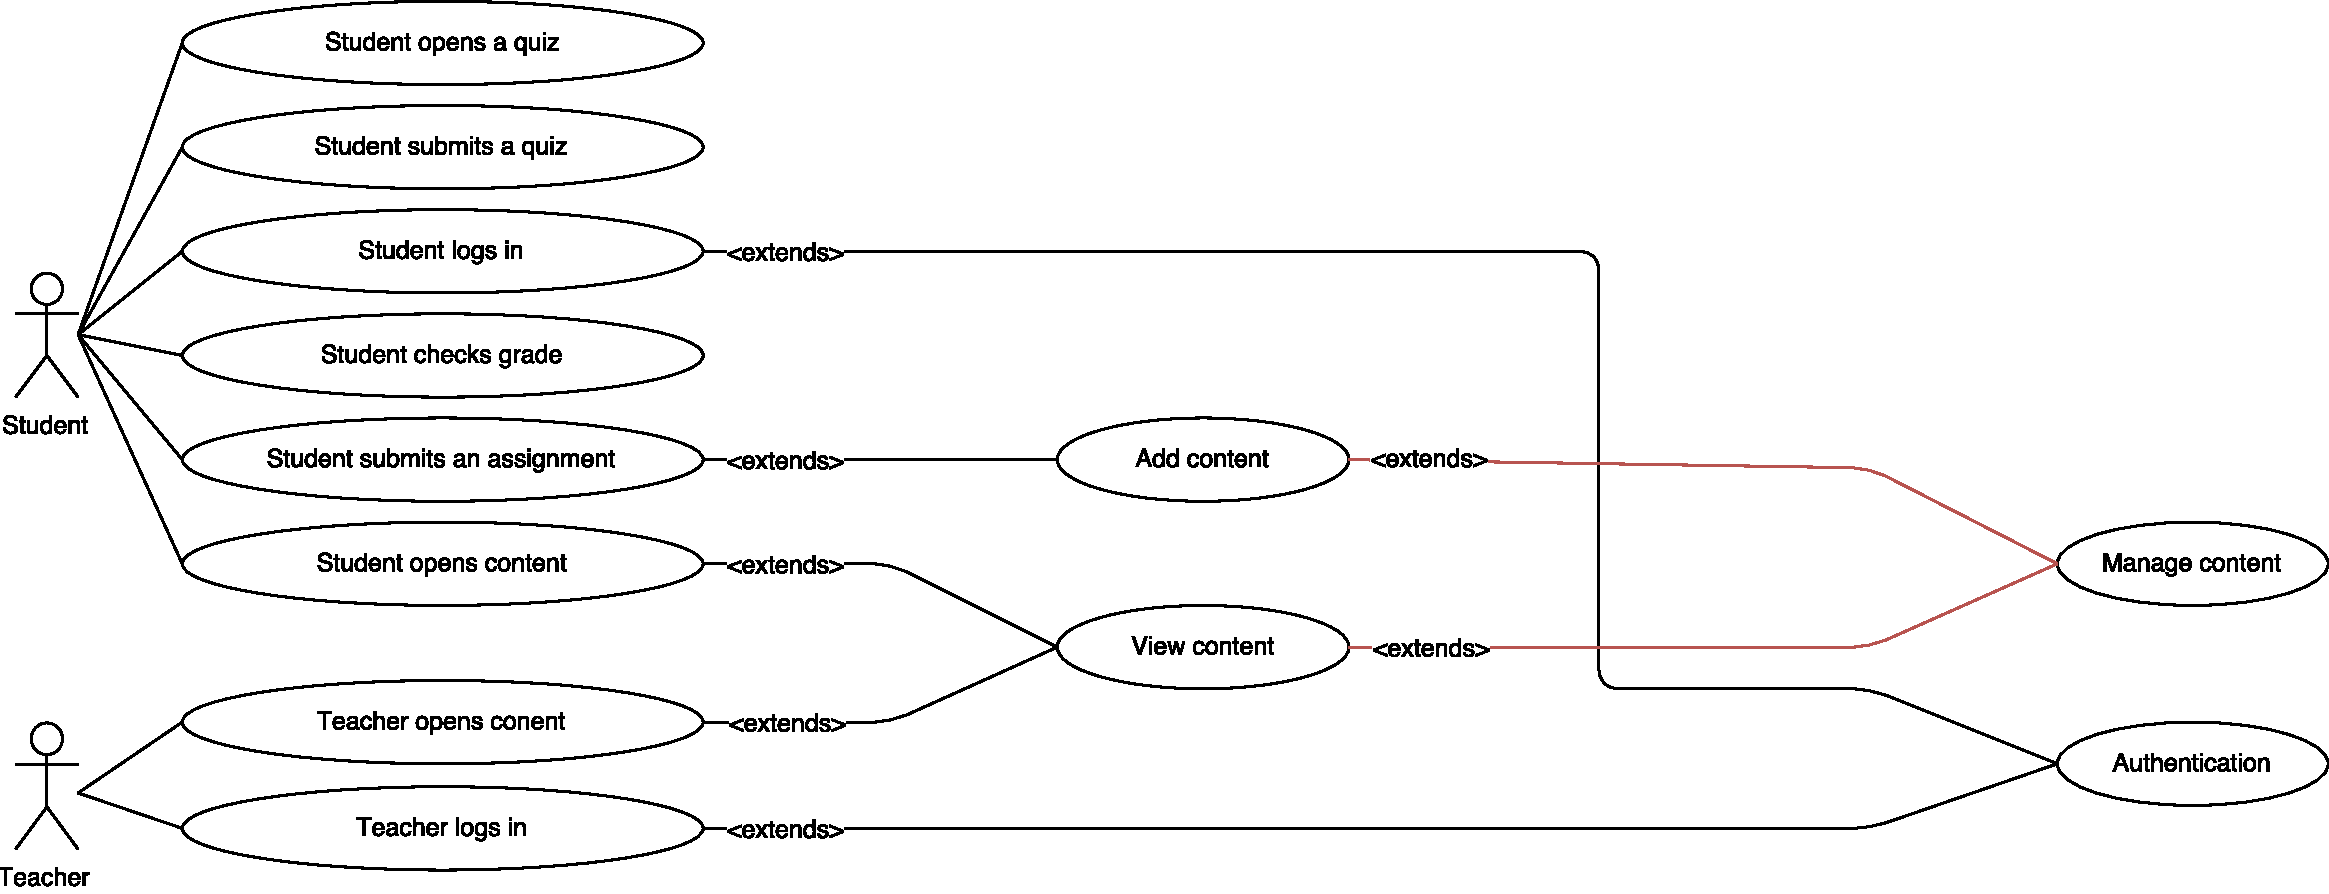
\includegraphics[scale=0.40]{A2_Assets/use_case_diagram.pdf}
  \caption{Use Case Diagram}
\end{figure}
}
Description:
\break \break 
 Student/Teacher logs in: The application takes the input credentials of the user and matches with credentials in servers. If authentication matches success message shown on screen. If not, no success message shown on screen.
 \hfill\break\break 
 Student opens a quiz: After being logged in the user selects to view quiz. Application downloads quiz from server and the application displays it to the user. The user is able to complete the quiz now. 
 \break\break 
 Student submits a quiz: The user completes their quiz and can now submit. Solutions of the quiz is downloaded from the server and marked by the application. Message is delivered to user displaying successful submission. 
 \break\break 
 Student opens content:
After being logged in the user selects to view content. Server downloads content from server and the application displays it to the user. The user is able to complete the assignment now. 
\break\break 
Teacher opens content:
After being logged in the user selects to view content. Server downloads content from server and the application displays it to the user.
\hfill\break\break 
Student submits an assignment: The user submits their assignment. There is a time stamp placed on the assignment. It is then uploaded to the server and a success message is displayed on the application.
\break\break 
Student checks grade:
After being logged in the user selects to view grades. The applications displays the grades of the user. 
 

\newpage

\section{Analysis Class Diagram}
\label{sec:analysis_class_diagram}
% Begin Section
The following diagram is an analysis class diagram for Erudite.\\

{
\begin{figure}[h]
  \centering
  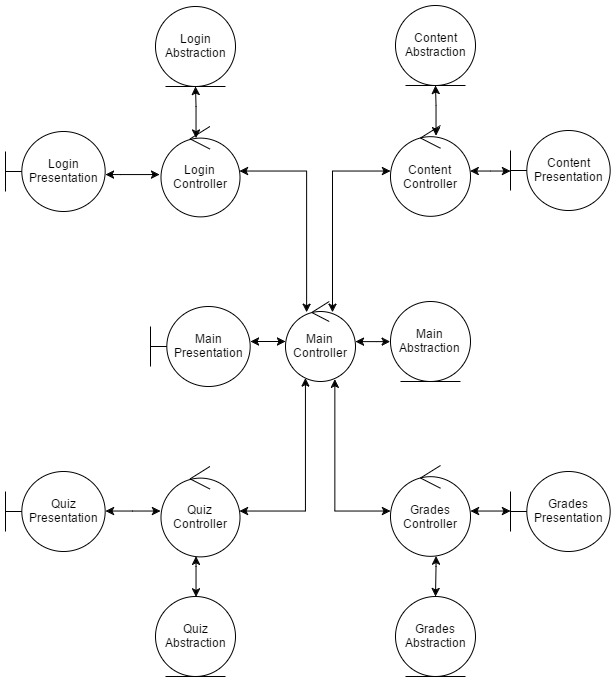
\includegraphics[scale=0.5]{A2_Assets/Analysis_Class_Diagrm_v3.jpg}
  \caption{Analysis Class Diagram}
\end{figure}
}


\section{Architectural Design}
\label{sec:architectural_design}
% Begin Section




\subsection{System Architecture}
\label{sub:system_architecture}
% Begin SubSection
Erudite will be built following the PAC architecture, where the system will be 
decomposed into a hierarchy of control modules, abstraction modules, and 
presentation modules.

The PAC architecture was chosen because Erudite is composed with multiple 
subsystems with interactive requirements. Each subsystem requires a view to 
display information, data which it processes for different users, and a 
controller to determine the sequence of events.

The main advantages of choosing the PAC architecture is it separates the 
different subsystems, and this allows for different people to implement the 
different subsystems independently of each other. Moreover, each component of 
the subsystem can also be separated so that each component can be implemented 
independently of each other.

Moreover, the PAC architecture allows dynamic view generation. Multiple views 
can be rendered onto the screen at the same time, and the user can select which 
views they want to see. The placement of different views can also be facilitated 
with the PAC architecture.

Furthermore, the PAC architecture allows for high cohesion and low coupling 
systems. The PAC architecture ensures high cohesion because each subsystem can 
only interact with the related components, and the main controller. This ensures 
that only relevant components are grouped together, and other components are 
grouped in other subsystems. Moreover, each of the systems only has a single 
connection to the main controller, and not to any other subsystems. Aside from 
the main controller, all of the subsystems are loosely coupled with each other, 
and the internal implementation of each subsystem can be changed with minimal 
modifications to the other subsystems.

Finally, the main controller in the PAC architecture allows Erudite to be 
extensible. New features can be added to the system with minimal modification: 
only a new Controller-Abstraction-Presentation needs to be added. Accordingly, 
Erudite will be based off the PAC architecture because of its ability to support 
multiple interactive subsystems while ensuring important software design 
principles such as high cohesion and low coupling.

%Add a structural architecture diagram here
{
  \begin{figure}[h]
  \centering
    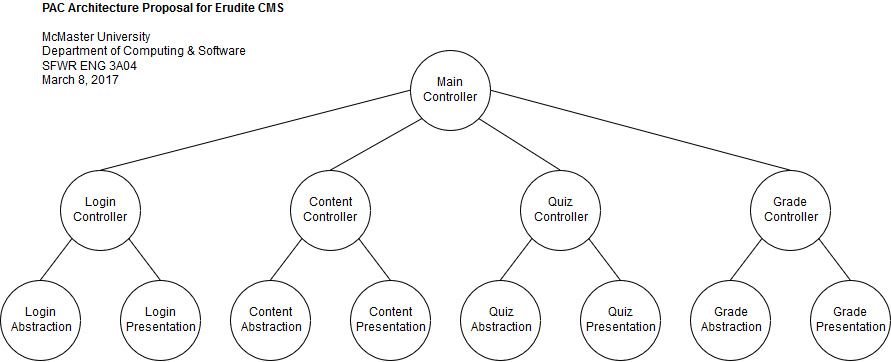
\includegraphics[scale=0.5]{A2_Assets/Structural_Class_Diagram_v3.jpg}
  \caption{Structural Architecture Diagram}
  \end{figure}
}
% End SubSection

\subsubsection{Comparison to Other Architectures}
While evaluating potential architectures for this project, the MVC-II 
architecture was also considered because it also supported views. However, the 
PAC architecture was ultimately chosen because of several inherent 
characteristics of the MVC-II architecture that made it less feasible to create 
the required application.

First, the MVC-II architecture only has one set of models, views, and 
controllers. With the requirement that the application must contain at least 3 
subsystems, restricting the application to only have one model, view, and 
controller would create a program with low cohesion: a single module would have 
to do many things.

Moreover, the MVC-II architecture also would not allow for different sets of 
data to be used for different purposes. The MVC-II architecture supports 
multiple views for a single dataset; however, our application has multiple sets 
of data: login credentials data, content data, quiz data, and grade data. 
Consolidating the different types of data into a single data store make the 
system less maintainable in the future.

Other architectures such as the blackboard architectures were considered; 
however, they were quickly rejected, as they did not support views and 
interactivity.

\subsection{Subsystems}
\label{sub:subsystems}
% Begin SubSection
\subsubsection{The Main Control Subsystem}
The purpose of this subsystem is to determine when each of the other subsystems 
is active, and displays the active subsystem's view to the main view. It 
receives view information from each of the 4 subsystems, and it is responsible 
for routing information between different systems.

\subsubsection{The Content Management System}
The purpose of the content management system is to receive and display content 
to the users. It sends view information to the main controller to be displayed, 
and it receives messages from the main control system in order to determine when 
to activate. 

\subsubsection{The Quiz Management System}
The purpose of the quiz management system is to receive and display 
automated-evaluational content to the users. This system randomly selects 
multiple-choice questions from a question bank, shuffles answers and displays 
them to the user. It is connected to the main control system which dictates when 
this 
system is active, and it sends requests to the main control to be forwarded to 
 to the main view for display.

\subsubsection{The Grade Management System}
The grade management system is responsible for receiving and displaying student 
grades to the users according to user type. The system displays only grades 
relevant to the student if a student accesses grades and displays all assigned 
grades to a teacher should a teacher access course grades. This system is 
connected to the main control system which dictates when this system is active, 
and 
it sends requests to the main control to be forwarded to the main view for 
display.

\subsubsection{The Authentication System}
The authentication system authenticates the users' login credentials. This 
system is 
connected to the control system which dictates when this system is active, and 
it sends requests to the main control to be forwarded view for display.

% End SubSection

% End Section

\section{Class Responsibility Collaboration (CRC) Cards}
\label{sec:class_responsibility_collaboration_crc_cards}
% Begin Section
The tables below show the Class Responsibility Collaboration cards for Erudite.
	
	 %New CRC
	
	%Main view
	\begin{table}[H]
	\centering
		\begin{tabular}{|p{9cm}|p{3cm}|}
		\hline
		 \multicolumn{2}{|l|}{\textbf{Class Name: Main View}} \\
		\hline
		\textbf{Responsibility:} & \textbf{Collaborators:} \\
		\hline
	    Display Login View & Login View, Login Controller, Main Controller\\
		\hline
		Display Content View & Content View, Content Controller, Main Controller 	\\
		\hline
		Display Quiz View & Quiz View, Quiz Controller, Main Controller\\
		\hline
		Display Grade View & Grade View, Grade Controller, Main Controller\\
		\hline 
		Displays data from Main Controller & Main Controller\\
		\hline
		Send content response to Main Controller & Main Controller\\
		\hline
		\end{tabular}
	\end{table}	
	
	%Main Controller
	\begin{table}[H]
	\centering
		\begin{tabular}{|p{9cm}|p{3cm}|}
		\hline
		 \multicolumn{2}{|l|}{\textbf{Class Name: Main Controller}} \\
		\hline
		\textbf{Responsibility:} & \textbf{Collaborators:} \\
		\hline
	    Receive request to validate login credentials & Login Controller\\
		\hline
	    Handle login validation requests & Main Abstraction\\
		\hline
		Receive authentication status information & Main Abstraction\\
		\hline
		Forward authentication status information & Login Controller\\
		\hline
		Receive request for quiz questions & Quiz Controller\\
		\hline
		Retrieve quiz questions & Main Abstraction \\
		\hline
		Receive quiz questions & Main Abstraction\\
		\hline
		Forward quiz questions & Quiz Controller\\
		\hline
		Receive quiz submission & Quiz Controller\\
		\hline
		Send request to grade quiz submission & Main Abstraction\\
		\hline
		Receive quiz results & Main Abstraction\\
		\hline
		Forward status code to indicate submission status & Quiz Controller\\
		\hline
		Receive content & Main Abstraction\\
		\hline
		Forward content & Content Controller\\
		\hline
		Forward user submitted content for storage & Main Abstraction\\
		\hline
		Receive request for user grades & Grade Controller\\
		\hline
		Receive user grades & Main Abstraction\\
		\hline
		Forward user grades & Grade Controller\\
		\hline
		\end{tabular}
	\end{table}
	
	%Main Abstraction
	\begin{table}[H]
	\centering
		\begin{tabular}{|p{9cm}|p{3cm}|}
		\hline
		 \multicolumn{2}{|l|}{\textbf{Class Name: Main Abstraction}} \\
		\hline
		\textbf{Responsibility:} & \textbf{Collaborators:} \\
		\hline
		Know how to access central data repository & Void\\
		\hline
		\end{tabular}
	\end{table}
	
	 %login view
	\begin{table}[H]
	\centering
		\begin{tabular}{|p{9cm}|p{3cm}|}
		\hline
		 \multicolumn{2}{|l|}{\textbf{Class Name: Login View}} \\
		\hline
		\textbf{Responsibility:} & \textbf{Collaborators:} \\
		\hline
		Request username and password pair from user & Login Controller\\
		\hline
		Receive authentication status & Logic Controller\\
		\hline
		Display authentication status & Void\\
		\hline
		\end{tabular}
	\end{table}
	
	 %login controller
	\begin{table}[H]
	\centering
		\begin{tabular}{|p{9cm}|p{3cm}|}
		\hline
		 \multicolumn{2}{|l|}{\textbf{Class Name: Login Controller}} \\
		\hline
		\textbf{Responsibility:} & \textbf{Collaborators:} \\
		\hline
	    Refactor login credentials & Login Abstraction\\
		\hline
		Forward authentication request for verification & Main Controller\\
		\hline
		Relay authentication status to the view & Login View\\
		\hline
		\end{tabular}
	\end{table}
	
	 %login abstraction
	\begin{table}[H]
	\centering
		\begin{tabular}{|p{9cm}|p{3cm}|}
		\hline
		 \multicolumn{2}{|l|}{\textbf{Class Name: Login Abstraction}} \\
		\hline
		\textbf{Responsibility:} & \textbf{Collaborators:} \\
		\hline
	    Know how to represent a user's username & Void\\
		\hline
		Know how to represent a user's password & Void\\
		\hline
		Know how to represent a username/password pair & Void\\
		\hline
		\end{tabular}
	\end{table}
	
	 %quiz view
	\begin{table}[H]
	\centering
		\begin{tabular}{|p{9cm}|p{3cm}|}
		\hline
		 \multicolumn{2}{|l|}{\textbf{Class Name: Quiz view}} \\
		\hline
		\textbf{Responsibility:} & \textbf{Collaborators:} \\
		\hline
		Request quiz questions & Quiz Controller\\
		\hline
	    Receive quiz questions & Quiz Controller\\
	    \hline
	    Display quiz questions & Void\\
	    \hline 
	    Request user attempt & Quiz Controller\\
	    \hline
	    Request to submit quiz from user& Quiz Controller\\
	    \hline
	    Receive submission status & Quiz Controller\\
	    \hline
	    Display submission status & Void\\
	    \hline
		\end{tabular}
	\end{table}
	
	 %quiz controller
	\begin{table}[H]
	\centering
		\begin{tabular}{|p{9cm}|p{3cm}|}
		\hline
		 \multicolumn{2}{|l|}{\textbf{Class Name: Quiz Controller}} \\
		\hline
		\textbf{Responsibility:} & \textbf{Collaborators:} \\
		\hline
	    Refactor quiz questions & Quiz Abstraction\\
		\hline
		Refactor submission notification & Quiz Abstraction\\
		\hline
	    Send request for quiz questions & Main Controller\\
		\hline
		Receive quiz questions & Main Controller\\
		\hline
		Forward quiz questions & Quiz View\\
		\hline
		Send quiz submission notification & Main Controller\\
		\hline
		Receive submission status & Main Controller\\
		\hline
		Forward submission status & Quiz View\\
		\hline
		\end{tabular}
	\end{table}
	
	 %quiz abstraction
	\begin{table}[H]
	\centering
		\begin{tabular}{|p{9cm}|p{3cm}|}
		\hline
		 \multicolumn{2}{|l|}{\textbf{Class Name: Quiz Abstraction}} \\
		\hline
		\textbf{Responsibility:} & \textbf{Collaborators:} \\
		\hline
	    Know how to represent quiz questions  & Void\\
		\hline
		Know how to represent quiz submission & Void\\
		\hline
		\end{tabular}
	\end{table}

	%Content view
	\begin{table}[H]
	\centering
		\begin{tabular}{|p{9cm}|p{3cm}|}
		\hline
		 \multicolumn{2}{|l|}{\textbf{Class Name: Content View}} \\
		\hline
		\textbf{Responsibility:} & \textbf{Collaborators:} \\
		\hline
		Receive request for content from user & Content Controller\\
		\hline
	    Receive content & Content Controller\\
	    \hline
	    Display content & Void\\
	    \hline 
	    Receive request for formatted content from user & Content Controller\\
	    \hline
	    Receive file submissions from the user & Content Controller\\
	    \hline
	    Receive formatted content & Content Controller\\
	    \hline
	    Display formatted content & Void\\
	    \hline
		\end{tabular}
	\end{table}
	
	 %Content controller
	\begin{table}[H]
	\centering
		\begin{tabular}{|p{9cm}|p{3cm}|}
		\hline
		 \multicolumn{2}{|l|}{\textbf{Class Name: Content Controller}} \\
		\hline
		\textbf{Responsibility:} & \textbf{Collaborators:} \\
		\hline
	    Refactor content & Content Abstraction\\
		\hline
		Refactor formatted content & Content Abstraction\\
		\hline
	    Send request for content & Main Controller\\
		\hline
		Receive content & Main Controller\\
		\hline
		Forward content & Content View\\
		\hline
		Forward formatted content & Content View\\
		\hline
		Forward user submissions & Main Controller\\
		\hline	
		\end{tabular}
	\end{table}
	
	 %Content abstraction
	\begin{table}[H]
	\centering
		\begin{tabular}{|p{9cm}|p{3cm}|}
		\hline
		 \multicolumn{2}{|l|}{\textbf{Class Name: Content Abstraction}} \\
		\hline
		\textbf{Responsibility:} & \textbf{Collaborators:} \\
		\hline
	    Know how to represent content  & Void\\
		\hline
		Know how to represented formatted content & Void\\
		\hline
		\end{tabular}
	\end{table}
	
	%Grade view
	\begin{table}[H]
	\centering
		\begin{tabular}{|p{9cm}|p{3cm}|}
		\hline
		 \multicolumn{2}{|l|}{\textbf{Class Name: Grade View}} \\
		\hline
		\textbf{Responsibility:} & \textbf{Collaborators:} \\
		\hline
		Request user grades and statistics & Grade Controller\\
		\hline
	    Receive user grades and statistics & Grade Controller\\
	    \hline
	    Display user grades and statistics& Void\\
	    \hline 
		\end{tabular}
	\end{table}
	
	 %Grade controller
	\begin{table}[H]
	\centering
		\begin{tabular}{|p{9cm}|p{3cm}|}
		\hline
		 \multicolumn{2}{|l|}{\textbf{Class Name: Grade Controller}} \\
		\hline
		\textbf{Responsibility:} & \textbf{Collaborators:} \\
		\hline
	    Refactor grades & Grade Abstraction\\
		\hline
		Refactor grade statistics & Grade Abstraction\\
		\hline
	    Request user grades & Main Controller\\
		\hline
		Receive user grades & Main Controller\\
		\hline
		Forward user grades & Grade View\\
		\hline
		Forward user grades statistics & Grade View\\
		\hline
		\end{tabular}
	\end{table}
	
	 %Grade abstraction
	\begin{table}[H]
	\centering
		\begin{tabular}{|p{9cm}|p{3cm}|}
		\hline
		 \multicolumn{2}{|l|}{\textbf{Class Name: Grade Abstraction}} \\
		\hline
		\textbf{Responsibility:} & \textbf{Collaborators:} \\
		\hline
	    Know how to represent grades  & Void\\
		\hline
		Know how to represent quiz statistics & Void\\
		\hline
		\end{tabular}
	\end{table}

% End Section

\newpage
\appendix
\section{Division of Labour}
\label{sec:division_of_labour}
\begin{description}
  \item [Kelvin Lin ]
  \item{Section 4.1}
  \item{Section 4.2}
  \item{General editing and formatting}
  \hfill \rule{2in}{0.1pt}
  \\\\

  \item [Danish Khan]
  \item{CRC Cards}
  \item{Structural Class Diagram}
  \hfill \rule{2in}{0.1pt}
  \\\\

  \item [Puru Jetly]
  \item{CRC Cards}
  \item{General editing and formatting}
  \hfill \rule{2in}{0.1pt}
  \\\\

  \item [Terrance Yip]
   \item{CRC Cards}
  \item{Analysis Class Diagram}
  \hfill \rule{2in}{0.1pt}
  \\\\

  \item [Varun Hooda]
  \item{Section 1 Introduction}
  \item{Revision to use case diagram}
  \hfill \rule{2in}{0.1pt}
  \\\\
\end{description}

\end{document}
%-----------------------------------------------------------------------------